\chapter{实验技术III：研究实践}\label{ch:b3:lab-techniques-3}

一瓶丁基锂溶液，只要有一滴接触空气便会起火；\omterm{def:b3:lab-techniques-3:schlenk}{手套箱}能
将氧气和水的含量控制在百万分之几以下，使此类化合物
可以像食盐一样称量。科研化学常始于隔绝空气，
终于一个必须能被他人核查的结论：
一种新化合物，其结构与纯度经多种独立方法证明，
其数据经记录并发表，以便工作可以重复。本章
汇集科研实践的操作：处理对空气敏感的物质、
表征新化合物、以统计方法判断结果、
管理\omterm{def:b3:lab-techniques-3:notebook}{实验记录本}并查阅文献，以及评估一项
此前无人进行过的操作的风险。

\begin{recall}
本科一年级分册讲述了危害、风险、象形图、H 和 P 说明、安全
技术说明书，以及测量不确定度的 A 类与 B 类评定；本科二年级分册
讲述了惰性气氛、后处理、干燥剂、快速柱色谱、
质谱法（HRMS、单同位素质量）、$^{13}$C 核磁共振谱、置信区间、
学生 t 系数、校准、精密度、正确度、偏倚、重复性、
方法验证、绝热温升与热失控。
\Cref{ch:b3:advanced-nmr}、\cref{ch:b3:x-ray-diffraction}和
\cref{ch:b3:electrode-kinetics}提供了结构与电化学
方法。
\end{recall}

\begin{omfigure}
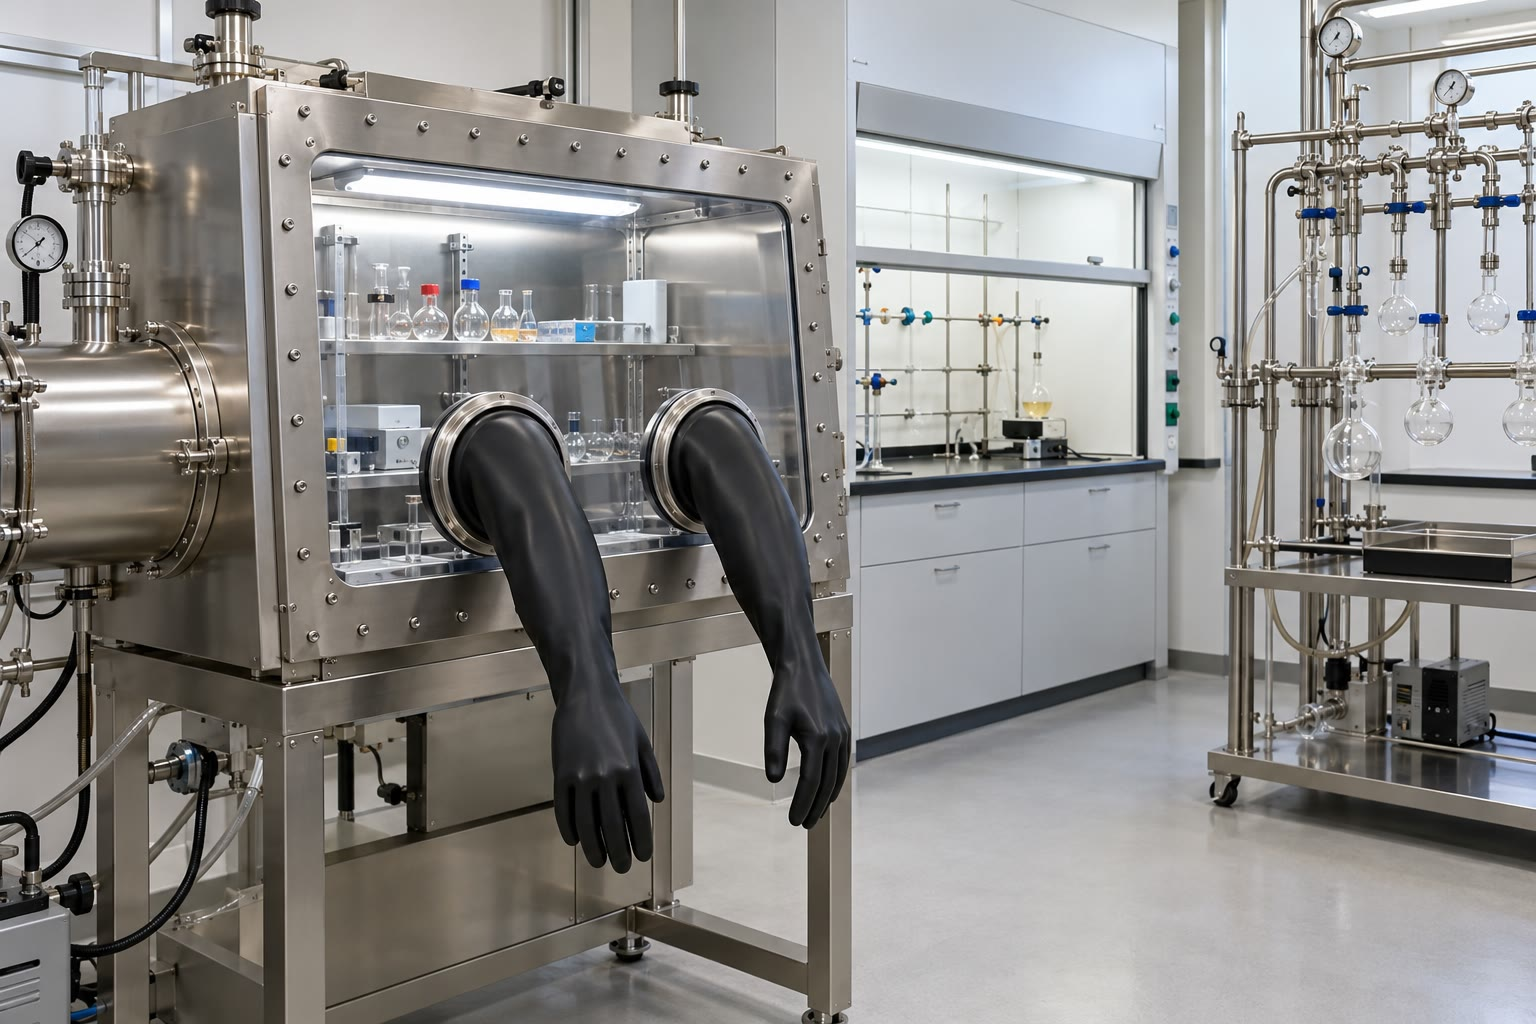
\includegraphics[width=0.58\linewidth]{images/book4/ai/b3-33-glovebox.jpg}

{\small 配有\omterm{def:b3:lab-techniques-3:schlenk}{手套箱}的科研实验室：不锈钢箱体，内充
干燥氮气或氩气，经手套进行操作；左侧的圆筒
为物品进出的过渡舱。}
\end{omfigure}

\section{无空气操作}

\begin{definition}[空气敏感化合物]\label{def:b3:lab-techniques-3:air-sensitive}
称能与空气中的氧气或水反应、发生分解或失去活性的
化合物为\emph{空气敏感化合物}\index{空气敏感化合物}。称
在空气中自发着火的物质为
\emph{自燃物质}\index{自燃物质}。
\end{definition}

\begin{definition}[希兰克线与手套箱]\label{def:b3:lab-techniques-3:schlenk}
称\emph{希兰克线}\index{希兰克线}为双管玻璃歧管，一管经
冷阱与真空泵相连，另一管与干燥惰性气体源相连，
经油泡器放空，并以旋塞使各接口可与
其中任一管相通。\emph{希兰克瓶}\index{希兰克瓶}带有一个
带旋塞的侧管，用于与线路相接。\emph{手套箱}\index{手套箱}是
一种密封箱体，内充惰性气体并持续净化，箱内操作借助
手套进行。
\end{definition}

\begin{omfigure}
\begin{tikzpicture}[font=\scriptsize, >=Stealth]
  % manifolds
  \draw[om glass, line width=1.1pt] (0,3.0) -- (8.0,3.0);
  \draw[om glass, line width=1.1pt] (0,2.5) -- (8.0,2.5);
  \node[anchor=east] at (-1.0,3.0) {惰性气体};
  \node[anchor=east] at (0,2.5) {真空};
  % taps
  \foreach \x in {2.0,4.0,6.0} {
    \draw[om glass] (\x,3.0) -- (\x,2.5);
    \draw[fill=white] (\x,2.75) circle (0.12);
    \draw (\x-0.1,2.75) -- (\x+0.1,2.75);
    \draw[om glass] (\x,2.5) -- (\x,2.0);
  }
  % flask on the middle tap
  \draw[thick, black!60] (4.0,2.0) -- (4.0,1.6) -- (4.6,1.6);
  \pic[scale=0.5, transform shape] at (5.0,-0.2) {rbflask={0.3}{omDef!20}};
  \draw[om glass] (4.6,1.6) -- (4.9,1.25);
  \node[anchor=west] at (5.4,0.4) {希兰克瓶};
  % bubbler at the gas end
  \pic[scale=0.55, transform shape] at (8.9,1.5) {bubbler};
  \draw[om glass] (8.0,3.0) -- (8.6,3.0) -- (8.6,2.9);
  \node[anchor=west] at (9.4,2.2) {油泡器};
  % trap and pump at the vacuum end
  \draw[om glass] (0.4,2.5) -- (0.4,1.6);
  \draw[om glass, fill=omDef!8] (0.15,1.6) rectangle (0.65,0.4);
  \fill[omDef!25] (0.0,0.2) rectangle (0.8,1.2);
  \node[anchor=north] at (0.4,0.2) {冷阱};
  \draw[om glass] (0.65,0.9) -- (1.6,0.9);
  \draw[fill=black!15] (1.6,0.6) rectangle (2.6,1.2);
  \node at (2.1,0.9) {泵};
  \draw[->, thick] (-0.9,3.0) -- (0,3.0);
\end{tikzpicture}

{\small \omterm{def:b3:lab-techniques-3:schlenk}{希兰克线}示意图：气体歧管与真空歧管通过
旋塞相连；每个旋塞使其所接烧瓶与真空或惰性气体
相通。溶剂蒸气被抽出后，在到达泵之前于冷阱中冷凝；
气体经油泡器排出，油泡器可阻止空气倒流。}
\end{omfigure}

\begin{proposition}[抽空–充气循环]\label{prop:b3:lab-techniques-3:purge-cycles}
若一个充满压强为 $p_0$ 空气的烧瓶，抽至 $p_{\min}$ 后充入
纯惰性气体，重复 $n$ 次，则残留的原有空气比例为 $(p_{\min}/p_0)^n$。
\end{proposition}

\begin{proof}
抽空至 $p_{\min}$ 后，剩余气体的比例为 $p_{\min}/p_0$，组成不变；
再充入纯惰性气体使压强恢复为 $p_0$，且不引入空气。每一循环使
空气比例乘以 $p_{\min}/p_0$；经 $n$ 次循环后，为 $(p_{\min}/p_0)^n$。
\end{proof}

按理论计算，三次循环至 \qty{0.1}{mbar} 后残留空气为 $10^{-12}$；实际上，漏气、
玻璃表面\omterm{def:b3:surfaces-catalysis:adsorption}{吸附}的气体以及真空脂与隔膜的放气决定了实际极限，
这也是玻璃仪器需在烘箱中烘干并趁热装配的原因。

\begin{definition}[套管转移]\label{def:b3:lab-techniques-3:cannula}
\emph{套管转移}\index{套管转移}是指将对空气敏感的液体，
借助长的双尖针头从一个密封容器转移至另一个，
转移的动力为第一个容器中少量惰性气体的超压。
\end{definition}

\begin{omfigure}
\begin{tikzpicture}[font=\scriptsize, >=Stealth]
  \pic at (0,0) {rbflask={0.35}{omThm!25}};
  \pic at (4.2,0) {rbflask={0.1}{omDef!15}};
  \pic at (0,3.0) {septum};
  \pic at (4.2,3.0) {septum};
  \draw[black!70, line width=0.9pt] (0.05,0.25) -- (0.05,3.5) to[out=90, in=90] (4.15,3.5) -- (4.15,1.6);
  \draw[->, thick, omThm] (1.3,3.95) -- (2.9,3.95) node[midway, above] {液体};
  \draw[->, thick] (-1.3,3.4) -- (-0.15,3.2) node[pos=0, left] {惰性气体入口（轻微超压）};
  \draw[->, thick] (4.35,3.2) -- (5.4,3.6) node[right] {排至鼓泡器};
  \node[anchor=north] at (0,-0.1) {源瓶};
  \node[anchor=north] at (4.2,-0.1) {接收瓶};
\end{tikzpicture}

{\small \omterm{def:b3:lab-techniques-3:cannula}{套管转移}示意：套管的下端伸入源瓶中的液体，
从源瓶通入的惰性气体将液体经套管压入接收瓶，
接收瓶经一根针头通向鼓泡器排气。}
\end{omfigure}

\begin{method}[套管转移]\label{met:b3:lab-techniques-3:cannula}
\begin{enumerate}
  \item 将两只带隔膜塞的烧瓶密封后，在\omterm{def:b3:lab-techniques-3:schlenk}{希兰克线}上置于惰性气体中。
  \item 用气体吹扫套管：将套管一端插入源瓶中液面上方，
        直至另一端有气体流出，再将该端插入接收瓶。
  \item 用针头为接收瓶放气；将套管的源端压入液面以下，
        超压驱动液体转移。
  \item 停止时，将针尖提至液面以上，先将套管从接收瓶中抽出，
        并立即在通风橱中先用干燥溶剂、后用水冲洗套管。
\end{enumerate}
\end{method}

\begin{definition}[冷冻–抽气–解冻脱气]\label{def:b3:lab-techniques-3:degassing}
\emph{冷冻–抽气–解冻脱气}\index{冷冻–抽气–解冻脱气}用于除去液体中的溶解气体：
先在液氮中冷冻液体，抽空其上方空间，
关闭活塞并使其解冻，使溶解气体逸入真空；
上述循环重复三次。
\end{definition}

干燥溶剂现在取自惰性气体保护下的活性氧化铝柱，
而不再使用钠存下的蒸馏装置。有机锂溶液的浓度会随时间下降，
因此使用前需要滴定，例如在干燥 THF 中用已称量的二苯乙酸进行滴定：
第一当量的有机锂使二苯乙酸去质子化，
稍过量的第一滴即生成黄色二价阴离子。

\begin{proposition}[有机锂的滴定度]\label{prop:b3:lab-techniques-3:titre}
若质量为 $m$ 的二苯乙酸（摩尔质量为 $M$）需消耗体积为 $V$ 的
有机锂溶液方能达到变色终点，则浓度为 $c = m/(MV)$。
\end{proposition}

\begin{proof}
在滴定终点之前，每个有机锂夺去酸中的一个质子；
酸耗尽时出现颜色变化。二者物质的量相等：$cV = m/M$。
\end{proof}

\begin{inthelab}[手套箱过渡舱]
物品须经过渡舱进入\omterm{def:b3:lab-techniques-3:schlenk}{手套箱}：先将物品放入舱内，
关闭外门，对舱室抽真空并充入箱内气体，
如此共进行三次；多孔物品因\omterm{def:b3:surfaces-catalysis:adsorption}{吸附}空气，须再长时间抽真空；
此后方可通过手套从箱内打开内门。溶剂
及敞口盛放的挥发性液体绝不可在过渡舱内抽真空，
凡会毒害净化柱的物质（如硫醇、卤代溶剂）
未经许可不得在箱内开启。
\end{inthelab}

\begin{omfigure}
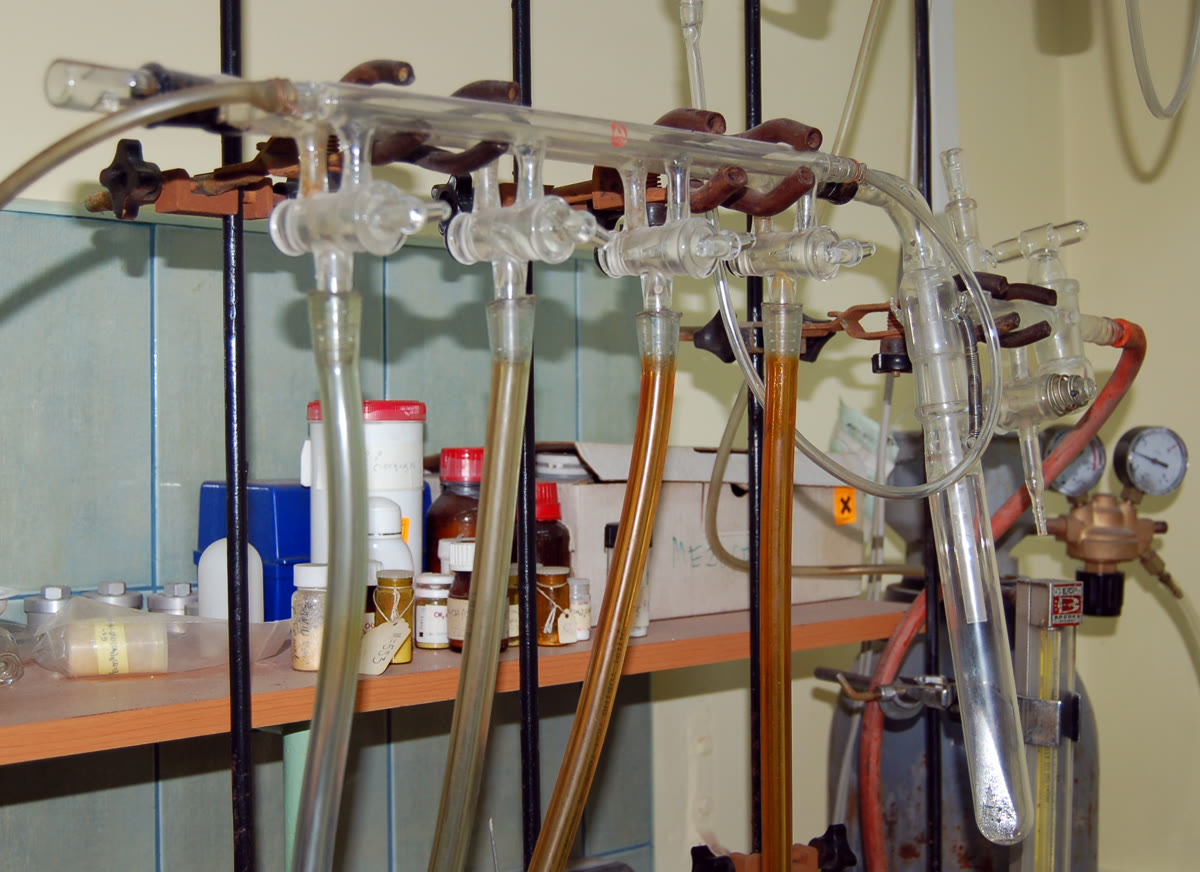
\includegraphics[width=0.46\linewidth]{images/book4/schlenk-line.jpg}

{\small 使用中的\omterm{def:b3:lab-techniques-3:schlenk}{希兰克线}：带活塞的玻璃歧管、通往烧瓶的
软管及气体调压器。照片：Polimerek，CC BY-SA 3.0。}
\end{omfigure}

\section{新化合物的表征}

\begin{method}[新化合物的表征]\label{met:b3:lab-techniques-3:characterise}
\begin{enumerate}
  \item 纯度：薄层色谱在两种洗脱剂中均为单一斑点，高效液相色谱或气相色谱为单一峰，
        熔点尖锐；若需质量纯度，则用\omterm{def:b3:lab-techniques-3:qnmr}{定量核磁共振}。
  \item 化学式：高分辨质谱（HRMS）测得质量与计算值相差在几个 ppm 之内，以及
        同位素峰形；或进行\omterm{def:b3:lab-techniques-3:elemental}{元素分析}。
  \item 结构：$^1$H 与 $^{13}$C 核磁共振及二维实验，用以确定连接方式
        （见\cref{ch:b3:advanced-nmr}），红外光谱用于确定官能团；若能长出晶体，
        则进行单晶 X 射线结构测定（见\cref{ch:b3:x-ray-diffraction}）。
  \item 立体化学：借助\omterm{def:b3:advanced-nmr:noe}{核欧沃豪斯效应}（NOE）、耦合常数和旋光度，
        以及手性色谱测定\omterm{def:b3:asymmetric-synthesis:ee}{对映体过量}（ee）。
  \item 报告每一项数据时须注明测定条件，谱图置于
        \omterm{def:b3:lab-techniques-3:literature}{补充材料}中。
\end{enumerate}
\end{method}

\begin{omfigure}
\begin{tikzpicture}[font=\scriptsize, >=Stealth,
  box/.style={draw, rounded corners, align=center, fill=omDef!8, inner sep=3pt, minimum height=8mm}]
  \node[box] (a) at (0,0) {新化合物 \\ 已分离};
  \node[box] (b) at (2.85,0) {纯度？\\ TLC、HPLC、熔点};
  \node[box] (c) at (5.85,0) {化学式 \\ HRMS、CHN};
  \node[box] (d) at (8.75,0) {结构 \\ NMR（一维、二维）、IR};
  \node[box] (e) at (8.75,-1.6) {有晶体则做 X 射线，\\ 立体化学};
  \node[box, fill=omMeth!12] (f) at (5.85,-1.6) {是否一致？\\ 连同原始数据 \\ 一并报告};
  \node[box, fill=omThm!10] (g) at (2.85,-1.6) {重新提纯 \\ （色谱、结晶）};
  \draw[->, thick] (a) -- (b); \draw[->, thick] (b) -- node[above, inner sep=1pt] {是} (c);
  \draw[->, thick] (c) -- (d); \draw[->, thick] (d) -- (e); \draw[->, thick] (e) -- (f);
  \draw[->, thick] (b) -- node[left] {否} (g); \draw[->, thick] (g.north west) to[bend left=30] (a.south);
\end{tikzpicture}

{\small 新化合物的表征流程：先看纯度，再定化学式，
最后确定结构；每项结论都须依赖至少两种独立方法，
并将\omterm{def:b3:lab-techniques-3:notebook}{原始数据}随报告一并提交。}
\end{omfigure}

\begin{definition}[元素分析]\label{def:b3:lab-techniques-3:elemental}
\emph{元素分析}\index{元素分析}（燃烧分析）用于测定样品中碳、氢、氮、硫的质量分数，
通过在氧气中燃烧样品，
测定生成的二氧化碳、水、氮气
与二氧化硫的量。
\end{definition}

\begin{proposition}[由化学式求质量分数]\label{prop:b3:lab-techniques-3:mass-fractions}
对化学式为 $\mathrm{C}_a\mathrm{H}_b\mathrm{N}_c\dots$、摩尔质量为 $M$ 的化合物，碳的质量分数为 $100\,aA_r(\mathrm C)/M$，
其他元素同理。
\end{proposition}

\begin{proof}
一摩尔化合物，质量为 $M$，含 $a$ 摩尔碳原子，其质量为 $aA_r(\mathrm C)$；
该比值乘以 100 即为质量分数。
\end{proof}

% ledger: ea:tolerance, hrms:tolerance
多数化学期刊要求，实测的 C、H、N 含量与计算值之差不超过
0.4 个百分点，或要求 HRMS 测得值在几个 ppm 以内（部分期刊为 5 ppm），
以此作为组成的证据。一项大型实验室间研究发现，即便是纯样品，
也常常出人意料地达不到 0.4 的判据，
这提醒我们判据并非自然定律。

\begin{proposition}[HRMS 误差]\label{prop:b3:lab-techniques-3:ppm-error}
测得质量 $m_{\mathrm{meas}}$ 相对于计算质量 $m_{\mathrm{calc}}$ 的误差为
$10^6(m_{\mathrm{meas}} - m_{\mathrm{calc}})/m_{\mathrm{calc}}$ ppm；对于离子，$m_{\mathrm{calc}}$ 由单同位素质量减去（或加上）
所移去（或加入）的电子质量而得。
\end{proposition}

\begin{proof}[由定义]
ppm 误差即以百万分之一表示的相对差；
离子质量与中性化学式质量的差来自电子，每个电子的质量为 \qty{5.486e-4}{u}，
在质量为几百时约为几个 ppm。
\end{proof}

\begin{definition}[定量核磁共振]\label{def:b3:lab-techniques-3:qnmr}
\emph{定量核磁共振}\index{定量核磁共振}（qNMR）通过信号积分确定物质的量或
纯度；信号积分与原子核数成正比，在脉冲间充分弛豫
条件下记录谱图时成立，并以与样品一同称量的
纯度已知的内标物为参照。
\end{definition}

\begin{proposition}[定量核磁共振纯度]\label{prop:b3:lab-techniques-3:qnmr}
设样品质量为 $m_x$，与质量为 $m_s$、纯度为 $P_s$ 的标准物一同称量，
信号积分分别为 $I_x$ 与 $I_s$，对应质子数为 $N_x$ 与 $N_s$，
\[
  P_x = \frac{I_x}{I_s}\,\frac{N_s}{N_x}\,\frac{M_x}{M_s}\,\frac{m_s}{m_x}\,P_s.
\]
\end{proposition}

\begin{proof}
积分与质子数成正比：$I_x/I_s = (N_xn_x)/(N_sn_s)$。
令 $n_x = P_xm_x/M_x$，$n_s = P_sm_s/M_s$，解出 $P_x$ 即得上式。
\end{proof}

\begin{omfigure}
\begin{tikzpicture}
\begin{axis}[width=0.8\linewidth, height=5.0cm, x dir=reverse, xmin=3.0, xmax=7.0, ymin=-0.05, ymax=1.15, clip=false,
  axis x line=bottom, axis y line=none, xlabel={化学位移 $\delta$ / ppm}, tick label style={font=\scriptsize}, label style={font=\small}]
\addplot[color=omDef, thick] table[x=ppm, y=y] {figdata/out/bachelor-3-qnmr.dat};
\node[font=\scriptsize, anchor=south] at (axis cs:6.09,0.33) {标准物，ArH（3 H）};
\node[font=\scriptsize, anchor=east] at (axis cs:4.20,0.98) {二茂铁（10 H）};
\node[font=\scriptsize, anchor=west, align=left] at (axis cs:3.72,0.70) {标准物，\\ $\ce{OCH3}$（9 H）};
\end{axis}
\end{tikzpicture}

{\small 二茂铁样品的模拟质子谱，样品与
1,3,5-三甲氧基苯为内标一同称量（模型：20.0 mg 样品，纯度 98.0\,\%
标准物 15.0 mg）。谱峰积分正比于
各化合物的质子数与其物质的量的乘积；
二茂铁单峰与标准物芳香单峰的积分之比给出纯度。}
\end{omfigure}

\section{科研结果的统计分析}

\begin{definition}[显著性检验]\label{def:b3:lab-techniques-3:tests}
\emph{显著性检验}\index{显著性检验}用于判断数据是否与
\emph{原假设}\index{原假设}相容，原假设通常是“无差异”或“无效应”，
在选定的、误拒原假设的风险水平下作出判断
（常取 5\,\%）。
\end{definition}

\begin{theorem}[双样本 $t$ 检验]\label{thm:b3:lab-techniques-3:t-test}
设两组相互独立的测量分别含 $n_1$ 与 $n_2$ 次，取自标准差相等的正态分布，
样本均值分别为 $\bar x_1$、$\bar x_2$，合并标准差为 $s_p$，
统计量 $t = (\bar x_1 - \bar x_2)/(s_p\sqrt{1/n_1 + 1/n_2})$ 在两真值相等时服从学生分布，
自由度为 $n_1 + n_2 - 2$。\admitted
\end{theorem}

\begin{proposition}[$F$ 检验]\label{prop:b3:lab-techniques-3:f-test}
在相同假设下，两样本方差之比 $F = s_1^2/s_2^2$ 服从
自由度为 $(n_1 - 1, n_2 - 1)$ 的费舍尔分布，前提是两真方差相等。
\admitted
\end{proposition}

\begin{method}[新方法的产率是否更高？]\label{met:b3:lab-techniques-3:compare-means}
\begin{enumerate}
  \item 在相同条件下将两种操作各重复数次，记录
        每一个结果。
  \item 先比较离散程度（$F$ 检验）；若两者相近，则合并：
        $s_p^2 = [(n_1 - 1)s_1^2 + (n_2 - 1)s_2^2]/(n_1 + n_2 - 2)$。
  \item 计算 $t$，并将 $|t|$ 与自由度为
        $n_1 + n_2 - 2$、选定水平下的学生 t 系数相比较。
  \item 更大则差异显著；更小则数据未显示差异，
        但这并不能证明不存在差异。
\end{enumerate}
\end{method}

可疑值绝不能因为不便而删除。离群值检验可以将其标出，
但取舍应依据\omterm{def:b3:lab-techniques-3:notebook}{实验记录本}：若有记录在案的原因（如称量失误、烧瓶受污染），
则可据此剔除；无此原因时，则保留该值，
或重做实验。

\section{实验记录本、科研数据与文献}

\begin{definition}[实验记录本与原始数据]\label{def:b3:lab-techniques-3:notebook}
\emph{实验记录本}\index{实验记录本}是按日期编写的、
连续且未经改动的实验记录，忠实反映实验的实际进行过程。\emph{原始数据}\index{原始数据}
是测量的原始记录（仪器文件、称量凭证、谱图），
均为未经任何加工的原始资料。
\end{definition}

\begin{method}[撰写实验记录条目]\label{met:b3:lab-techniques-3:notebook}
\begin{enumerate}
  \item 日期、标题、目的，以及对前一相关实验的引用。
  \item 反应方案及各物质的用量（质量、体积、摩尔数、当量），
        试剂来源与批号，以及\omterm{def:b3:lab-techniques-3:assessment}{风险评估}。
  \item 所做操作与观察现象，按先后顺序并标明时间，包括出错之处
        ；不得擦除，应以单线划改，使原记录仍清晰可辨。
  \item 结果：产率、\omterm{def:b3:lab-techniques-3:notebook}{原始数据}文件名称及结论；并签名。
\end{enumerate}
\end{method}

\begin{definition}[FAIR 数据]\label{def:b3:lab-techniques-3:fair}
% ledger: fair:year
\emph{FAIR 数据}\index{FAIR 数据}是科研数据，具有可查找、可获取、
可互操作和可重用的特性：附有丰富的元数据和
持久标识符，可通过标准协议检索，采用开放格式，
并附明确的许可证与来源信息。
\end{definition}

\begin{definition}[科研诚信]\label{def:b3:lab-techniques-3:integrity}
\emph{科研诚信}\index{科研诚信}是指科研的实施与成果报告须坚持诚实、
透明的行为规范。其最严重的违背行为包括
\emph{捏造}\index{捏造}（编造数据），\emph{篡改}\index{篡改}
（改动数据、图像或操作过程）和\emph{剽窃}\index{剽窃}
（将他人成果据为己有）。
\end{definition}

\begin{definition}[文献]\label{def:b3:lab-techniques-3:literature}
\emph{一次文献}\index{一次文献}报道原始研究成果，
包括论文、专利和学位论文；\emph{二次文献}\index{二次文献}
对其进行评述与整理，包括综述、手册、数据库，
教科书则构成第三层。\emph{同行评议}\index{同行评议}是指独立专家
在论文发表前对稿件所作的评审。文章的
\emph{补充材料}\index{补充材料}载有使他人重复
和检验工作所需的实验细节与
数据。
\end{definition}

\begin{method}[阅读已发表的实验方法]\label{met:b3:lab-techniques-3:read-paper}
\begin{enumerate}
  \item 阅读实验部分及\omterm{def:b3:lab-techniques-3:literature}{补充材料}，而不只是
        摘要和反应方案。
  \item 核查规模、浓度、温度、时间和后处理，并记下
        缺失的内容。
  \item 对照上文方法核查生成物的表征。
  \item 查找此后使用或修正了该方法的文献；
        应先在小规模下试做。
\end{enumerate}
\end{method}

结构数据库与反应数据库按化合物和转化过程为\omterm{def:b3:lab-techniques-3:literature}{一次文献}建立索引，
检索时不靠文字关键词，而是通过绘制结构式
或反应式进行检索。

\section{新实验步骤的风险评估}

\begin{definition}[风险评估]\label{def:b3:lab-techniques-3:assessment}
\emph{风险评估}\index{风险评估}是指对某一步骤识别其
危害，估计在计划条件下造成伤害的可能性与严重程度，
并设定能将风险降至可接受水平的控制措施。
\emph{控制层级}\index{控制层级}将这些措施按有效性从高到低排列：
消除、替代、工程控制、
管理控制、个人防护装备。
\end{definition}

\begin{omfigure}
\begin{tikzpicture}[font=\scriptsize]
  \foreach \i/\lab/\col in {0/消除：去除危害/omMeth!40, 1/替代：改用危害较小的试剂/omMeth!28, 2/{工程控制：通风橱、手套箱、防护屏}/omDef!22, 3/{管理控制：规程、培训}/omProp!22, 4/个人防护装备/omThm!22} {
    \pgfmathsetmacro\w{5.4-0.95*\i}
    \fill[\col] ({-\w/2},{-0.75*\i}) -- ({\w/2},{-0.75*\i}) -- ({\w/2-0.475},{-0.75*\i-0.7}) -- ({-\w/2+0.475},{-0.75*\i-0.7}) -- cycle;
    \node[anchor=west] at (3.0,{-0.75*\i-0.35}) {\lab};
    \draw[black!30] ({\w/2-0.2},{-0.75*\i-0.35}) -- (2.95,{-0.75*\i-0.35});
  }
  \node[anchor=east, align=right] at (-2.9,-0.35) {效果最好};
  \node[anchor=east, align=right] at (-2.9,-3.35) {效果最差};
  \draw[->, black!50] (-3.3,-0.85) -- (-3.3,-2.85);
\end{tikzpicture}

{\small \omterm{def:b3:lab-techniques-3:assessment}{控制层级}以倒金字塔表示：消除或替代危害
对所有人始终起保护作用；个人防护装备仅保护
其穿戴者，且仅在穿戴并完好时有效。}
\end{omfigure}

\begin{definition}[过氧化物形成剂]\label{def:b3:lab-techniques-3:peroxide}
\emph{过氧化物形成剂}\index{过氧化物形成剂}是一类化合物，如乙醚、四氢呋喃
或 1,4-二氧六环，在储存时与空气缓慢生成易爆过氧化物，
尤其是开封后及在光照下。
\end{definition}

\begin{method}[评估新实验步骤的风险]\label{met:b3:lab-techniques-3:risk-assessment}
\begin{enumerate}
  \item 列出所有物质（试剂、溶剂、生成物、副产物、释放的气体）
        及其安全技术说明书中给出的危害。
  \item 列出各操作及其条件（加热、压力、规模、
        淬灭、废物处理），估算放出的热量与
        绝热温升，然后再放大规模。
  \item 针对每种危害，按\omterm{def:b3:lab-techniques-3:assessment}{控制层级}由高到低选择措施；规划应急响应
        （泄漏、着火、接触）及废物处置途径。
  \item 书面记录，经他人核查，并在首次实施后复核。
\end{enumerate}
\end{method}

\begin{safety}{\ghs[0.62cm]{GHS02}\ghs[0.62cm]{GHS05}\ghs[0.62cm]{GHS07}\ghs[0.62cm]{GHS08}}
% ledger: ghs4:BuLi, ghs4:Et2O, ghs4:THF
丁基锂溶液为\omterm{def:b3:lab-techniques-3:air-sensitive}{自燃物质}，遇水剧烈反应并放出易燃气体，
造成严重灼伤；只能在惰性气体下操作，并备好干砂桶，附近不得有水。
氢化钠同样遇水和湿气放出氢气，常以油分散体形式使用。
乙醚与四氢呋喃为高度易燃的\omterm{def:b3:lab-techniques-3:peroxide}{过氧化物形成剂}：
开封时须标注日期，蒸馏或蒸发前须检测过氧化物，
并按期废弃。
\end{safety}

\begin{history}[施莱克的玻璃仪器]
威廉·施莱克于 1910 年代研究有机碱金属化合物与自由基，
设计了使其能在无空气条件下操作的烧瓶与技术，
今天的\omterm{def:b3:lab-techniques-3:schlenk}{希兰克线}与\omterm{def:b3:lab-techniques-3:schlenk}{希兰克瓶}仍以他的名字命名。第一批\omterm{def:b3:lab-techniques-3:schlenk}{手套箱}于
1940 年代为放射性材料而制造，不久后被
从事\omterm{def:b3:lab-techniques-3:air-sensitive}{空气敏感化合物}研究的化学家采用。
\end{history}

\section{练习}

\begin{exercise}[$\star$]\label{exo:b3:lab-techniques-3:1}
将烧瓶抽真空至 \qty{0.50}{mbar}，再充入氩气至 \qty{1013}{mbar}，重复三次。理论上，
原有空气的残留比例为多少？实际上什么因素限制了结果？
\end{exercise}

\begin{exercise}[$\star$]\label{exo:b3:lab-techniques-3:2}
丁基锂溶液的滴定度为 \qty{1.48}{mol/L}。需转移多大体积，
才能提供 \qty{20.0}{mmol}？
\end{exercise}

\begin{exercise}[$\star$]\label{exo:b3:lab-techniques-3:3}
% ledger: mass:C12, mass:H1, mass:Fe56, const4:me.u, hrms:tolerance
由单同位素质量计算二茂铁自由基阳离子 $\ce{C10H10Fe+}$ 的精确质量，
（$^{12}$C 精确为 12，$^1$H 为 1.00782503，$^{56}$Fe 为 55.93493633，电子质量为 \qty{5.486e-4}{u}），并求测得值
186.0129 的误差（以 ppm 计）。
\end{exercise}

\begin{exercise}[$\star$]\label{exo:b3:lab-techniques-3:4}
将下列文献分类为\omterm{def:b3:lab-techniques-3:literature}{一次文献}、\omterm{def:b3:lab-techniques-3:literature}{二次文献}或三次文献：综述文章、
报道新合成方法的期刊论文、专利、物理常数手册、
学位论文、教科书。
\end{exercise}

\begin{exercise}[$\star\star$]\label{exo:b3:lab-techniques-3:5}
% ledger: ea:tolerance
计算咖啡因 $\ce{C8H10N4O2}$ 的 C、H、N 质量分数，并判断实测值
C 49.31、H 5.22、N 28.71\,\% 是否符合通常的 0.4 个百分点判据。
\end{exercise}

\begin{exercise}[$\star\star$]\label{exo:b3:lab-techniques-3:6}
取 \qty{170.0}{mg} 二苯乙酸（$\ce{C14H12O2}$）试样，滴定至黄色终点
需 \qty{0.54}{mL} 丁基锂溶液。求其滴定度。
\end{exercise}

\begin{exercise}[$\star\star$]\label{exo:b3:lab-techniques-3:7}
旧方法得产率为 72、75、71、74 和 73\,\%；改进方法为 76、78、75、77 和
79\,\%。已知 8 个自由度、95\,\% 置信水平下的学生 t 系数为 2.31（数据见本题），
判断改进是否显著。
\end{exercise}

\begin{exercise}[$\star\star$]\label{exo:b3:lab-techniques-3:8}
两种方法各得六个结果，标准差分别为 0.80 与 0.30（
单位相同）。已知 (5, 5) 个自由度、95\,\% 置信水平下的临界 $F$ 值为 5.05（
数据见本题），判断二者的精密度是否存在差异。
\end{exercise}

\begin{exercise}[$\star\star$]\label{exo:b3:lab-techniques-3:9}
拟定实验室四氢呋喃与乙醚试剂瓶的
储存与检测方案。
\end{exercise}

\begin{exercise}[$\star\star\star$]\label{exo:b3:lab-techniques-3:10}
某学生拟在 60 °C 下于 DMF 中用氢化钠使一种醇去质子化，
规模为 50 g。请指出其中的危害（包括该溶剂与
碱共存时的热危害），并按\omterm{def:b3:lab-techniques-3:assessment}{控制层级}选择控制措施。
\end{exercise}

\begin{exercise}[$\star\star\star$]\label{exo:b3:lab-techniques-3:11}
将 $I_x$、$I_s$（各为 0.50\,\%）、$m_x$ 与 $m_s$（质量分别为 20.0
与 15.0 mg，二者不确定度均为 \qty{0.010}{mg}）以及 $P_s$（0.10\,\%）的相对标准不确定度，传递至\omterm{def:b3:lab-techniques-3:qnmr}{定量核磁共振}公式，并给出 $P_x$ 的相对不确定度。
哪一项占主导？
\end{exercise}

\begin{exercise}[$\star\star\star$]\label{exo:b3:lab-techniques-3:12}
五次滴定所得体积（单位 mL）为 81.2、82.0、80.6、81.5 和 89.0。用狄克逊检验得
$Q = 0.83$，临界值为 0.71（数据见本题）。最后一个数值是否应
舍弃？请说明你首先会检查什么。
\end{exercise}

\section{问题：从烧瓶到纸面}

\begin{problem}[{周末问题——从烧瓶到纸面：一种新的空气敏感化合物，
即在氮气下合成二茂铁、对其进行表征，
用定量核磁共振测定其纯度，并对该操作进行风险评估}]
\label{pb:b3:lab-techniques-3:1}
% ledger: aw:C, aw:H, aw:Fe, aw:Cl, aw:O, mass:C12, mass:H1, mass:Fe56, const4:me.u, ghs4:ferrocene
题目数据。无水氯化铁（II）（5.00 g）与环戊二烯负离子钠
（两当量，由环戊二烯与氢化钠在四氢呋喃中制得）在氮气下反应；
分离得到 5.86 g 橙色二茂铁 $\ce{Fe(C5H5)2}$。反应瓶
经三个循环置换，每次由 \qty{1000}{mbar} 抽至 \qty{0.10}{mbar}。高分辨质谱给出 $m/z$ 为 186.0129（对应 $\ce{M+}$）；\omterm{def:b3:lab-techniques-3:elemental}{元素分析}结果
为 C 64.41、H 5.47\,\%。在 $\ce{CDCl3}$ 中，二茂铁于 4.16 ppm 处给出一个单峰（10 H）。进行\omterm{def:b3:lab-techniques-3:qnmr}{定量核磁共振}时，
取 20.0 mg 样品与 15.0 mg 的 1,3,5-三甲氧基苯（纯度 99.9\,\%，芳香单峰位于
6.09 ppm 处，3 H）混合，得 $I_x/I_s = 3.942$；每个积分的相对标准不确定度为 0.50\,\%，
每个质量的标准不确定度为 \qty{0.010}{mg}，$P_s$ 的相对标准不确定度为 0.10\,\%。

\medskip\noindent\textbf{第一部分——氮气下的合成。}
\begin{enumerate}
  \item 写出合成反应方程式。
  \item 为何反应必须在无空气条件下进行？
  \item 计算二茂铁的理论质量及产率。
  \item 计算经三个置换循环后残留空气的比例。
  \item 如何由环戊二烯二聚体得到环戊二烯？为何必须立即使用？
  \item 为何氢化钠要分批加入？
\end{enumerate}

\medskip\noindent\textbf{第二部分——表征。}
\begin{enumerate}[resume]
  \item 计算 $\ce{M+}$ 的精确质量，并求测量误差（以 ppm 计）。
  \item 计算 C、H 的质量分数，并与\omterm{def:b3:lab-techniques-3:elemental}{元素分析}结果比较。
  \item 为何二茂铁只显示一个 $^1$H 信号？
  \item $^{13}$C 核磁共振谱会显示什么？
  \item 还需要哪种方法来证明夹心结构？
  \item 二茂铁制得后本身是否对空气敏感？请与其前体比较。
\end{enumerate}

\medskip\noindent\textbf{第三部分——\omterm{def:b3:lab-techniques-3:qnmr}{定量核磁共振}测纯度。}
\begin{enumerate}[resume]
  \item 此处为何选择 1,3,5-三甲氧基苯作为标准物？
  \item 核磁共振采集须保证哪些条件，积分才具有定量意义？
  \item 计算二茂铁与标准物的摩尔质量。
  \item 计算样品的纯度。
  \item 计算其相对标准不确定度与绝对标准不确定度。
  \item \omterm{def:b3:lab-techniques-3:elemental}{元素分析}结果是否与该纯度相符？
\end{enumerate}

\medskip\noindent\textbf{第四部分——风险与最后一次测量。}
\begin{enumerate}[resume]
  \item 列出该操作的危害。
  \item 为氢化钠与四氢呋喃选择控制措施。
  \item 反应结束时，过量的氢化钠应如何销毁？
  \item 二茂铁的循环\omterm{def:b3:electrode-kinetics:cv}{伏安图}显示什么，为何
        电化学中用二茂铁作参比？
  \item \omterm{def:b3:lab-techniques-3:notebook}{实验记录本}与\omterm{def:b3:lab-techniques-3:literature}{补充材料}须包含哪些内容？
  \item 为何原始谱图应以开放格式归档？
  \item 给出结果：二茂铁样品的\omterm{def:b3:lab-techniques-3:qnmr}{定量核磁共振}纯度及其标准
        不确定度。
\end{enumerate}
\end{problem}
